\documentclass[remotesensing,article,submit,pdftex,moreauthors]{Definitions/mdpi} 


%=================================================================
% MDPI internal commands
\firstpage{1} 
\makeatletter 
\setcounter{page}{\@firstpage} 
\makeatother
\pubvolume{1}
\issuenum{1}
\articlenumber{0}
\pubyear{2022}
\copyrightyear{2022}
%\externaleditor{Academic Editor: Firstname Lastname} % For journal Automation, please change Academic Editor to "Communicated by"
\datereceived{} 
\dateaccepted{} 
\datepublished{} 
%\datecorrected{} % Corrected papers include a "Corrected: XXX" date in the original paper.
%\dateretracted{} % Corrected papers include a "Retracted: XXX" date in the original paper.
\hreflink{https://doi.org/} % If needed use \linebreak
%\doinum{}
%------------------------------------------------------------------
% The following line should be uncommented if the LaTeX file is uploaded to arXiv.org
%\pdfoutput=1

%=================================================================
% Add packages and commands here. The following packages are loaded in our class file: fontenc, inputenc, calc, indentfirst, fancyhdr, graphicx, epstopdf, lastpage, ifthen, lineno, float, amsmath, setspace, enumitem, mathpazo, booktabs, titlesec, etoolbox, tabto, xcolor, soul, multirow, microtype, tikz, totcount, changepage, attrib, upgreek, cleveref, amsthm, hyphenat, natbib, hyperref, footmisc, url, geometry, newfloat, caption
%=================================================================
%% Please use the following mathematics environments: Theorem, Lemma, Corollary, Proposition, Characterization, Property, Problem, Example, ExamplesandDefinitions, Hypothesis, Remark, Definition, Notation, Assumption
%% For proofs, please use the proof environment (the amsthm package is loaded by the MDPI class).

%=================================================================
% Full title of the paper (Capitalized)
\Title{Robot Team II: Electric Boogaloo}

% MDPI internal command: Title for citation in the left column
\TitleCitation{Robot Team II: Electric Boogaloo}

% Author Orchid ID: enter ID or remove command
\newcommand{\orcidauthorA}{0000-0002-5910-0183} % Add \orcidA{} behind the author's name
\newcommand{\orcidauthorB}{0000-0000-0000-000X} % Add \orcidB{} behind the author's name

% Authors, for the paper (add full first names)
% \Author{John Waczak $^{1,\dagger,\ddagger}$\orcidA{} and David J. Lary $^{1,\ddagger}$\orcidB{}}
\Author{John Waczak\orcidA{} and David J. Lary\orcidB{}}

%\longauthorlist{yes}

% MDPI internal command: Authors, for metadata in PDF
\AuthorNames{John Waczak and David J. Lary}

% MDPI internal command: Authors, for citation in the left column
\AuthorCitation{Waczak, J.; Lary, D.J.}
% If this is a Chicago style journal: Lastname, Firstname, Firstname Lastname, and Firstname Lastname.

% Affiliations / Addresses (Add [1] after \address if there is only one affiliation.)
\address{%
  Hanson Center for Space Sciences, University of Texas at Dallas, Richardson,
  TX 75080, USA;}

% $^{1}$ \quad John.Waczak@utdallas.edu\\
% $^{2}$ \quad David.Lary@utdallas.edu}

% Contact information of the corresponding author
\corres{Correspondence: John.Waczak@utdallas.edu}

% Current address and/or shared authorship
%\firstnote{}
% \secondnote{These authors contributed equally to this work.}
% The commands \thirdnote{} till \eighthnote{} are available for further notes

%\simplesumm{} % Simple summary

%\conference{} % An extended version of a conference paper

% Abstract (Do not insert blank lines, i.e. \\)
\abstract{A robust characterization of model uncertainties is critical for any time-sensitive or dangerous application...To that end we employ a combination of model stacking together with Conformal Prediction by which we are able to blend together a variety of ML models while simultaneously estimating confidence intervals for the resulting predictions. }

% Keywords
\keyword{Remote Sensing; hyperspectral image; georectification; machine learning}

% The fields PACS, MSC, and JEL may be left empty or commented out if not applicable
%\PACS{J0101}
%\MSC{}
%\JEL{}

%%%%%%%%%%%%%%%%%%%%%%%%%%%%%%%%%%%%%%%%%%
% Only for the journal Diversity
%\LSID{\url{http://}}

%%%%%%%%%%%%%%%%%%%%%%%%%%%%%%%%%%%%%%%%%%
% Only for the journal Applied Sciences:
%\featuredapplication{Authors are encouraged to provide a concise description of the specific application or a potential application of the work. This section is not mandatory.}
%%%%%%%%%%%%%%%%%%%%%%%%%%%%%%%%%%%%%%%%%%

%%%%%%%%%%%%%%%%%%%%%%%%%%%%%%%%%%%%%%%%%%
% Only for the journal Data:
%\dataset{DOI number or link to the deposited data set in cases where the data set is published or set to be published separately. If the data set is submitted and will be published as a supplement to this paper in the journal Data, this field will be filled by the editors of the journal. In this case, please make sure to submit the data set as a supplement when entering your manuscript into our manuscript editorial system.}

%\datasetlicense{license under which the data set is made available (CC0, CC-BY, CC-BY-SA, CC-BY-NC, etc.)}

%%%%%%%%%%%%%%%%%%%%%%%%%%%%%%%%%%%%%%%%%%
% Only for the journal Toxins
%\keycontribution{The breakthroughs or highlights of the manuscript. Authors can write one or two sentences to describe the most important part of the paper.}

%%%%%%%%%%%%%%%%%%%%%%%%%%%%%%%%%%%%%%%%%%
% Only for the journal Encyclopedia
%\encyclopediadef{Instead of the abstract}
%\entrylink{The Link to this entry published on the encyclopedia platform.}
%%%%%%%%%%%%%%%%%%%%%%%%%%%%%%%%%%%%%%%%%%
\begin{document}

%%%%%%%%%%%%%%%%%%%%%%%%%%%%%%%%%%%%%%%%%%
\section{Introduction}

\subsection{Importance / Human Impact}
oil spill response, contaminated water, environmental surveys, algal blooms,
agriculture, land monitoring, air quality, etc...

paper using spectral indices for water quality assesment \cite{SpectralIndexWaterQuality}


\subsection{Hyperspectral Imaging and Remote Sensing}
paper creating new spectral index for wheat rust \cite{SpectralIndexWheat} \\ 
overview of NDVI \cite{SpectralIndexNDVI} \\ 
paper using spectral indices for desertification \cite{SpectralIndexDesertification}


\subsubsection{HSI sattelite systems}
\subsubsection{HSI drone systems}
\subsubsection{Machine Learning using HSI}
add Xiao He reference here \cite{yu2021pm2}

\subsection{In-situ Measurements / Robot Teams}
\subsubsection{Meteorology}
\subsubsection{Atmospheric Sensing}
add in reference to our AQ sensor network

\subsection{Julia Programming Language}
\subsubsection{scientific computing}
\subsubsection{differentiable programming ($\partial P$)}
\subsubsection{MLJ}
discuss general \textit{learning network} framework and utilization of
Directed Acyclic Graphs for pipeline construction

basic overview of MLJ as a Julia package \cite{MLJ1}\\ 

detailed description of \textit{learning networks} \cite{MLJ2}


\section{Materials and Methods}
\subsection{Autonomous Collection and Processing of Hyperspectral Images}

website for alta x \cite{freeflyAltaX}


\begin{figure}[H]
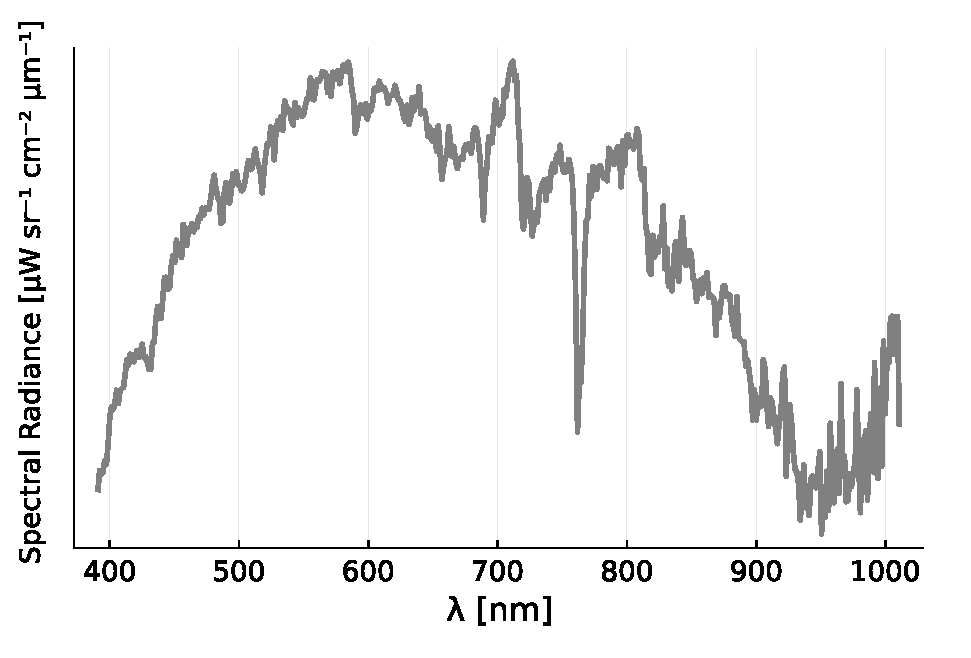
\includegraphics[width=10.5 cm]{images/spectra/radiance.eps}
\caption{Spectral Radiance collected from a single pixel of the HSI.\label{radiancePlot}}
\end{figure}   

\begin{figure}[H]
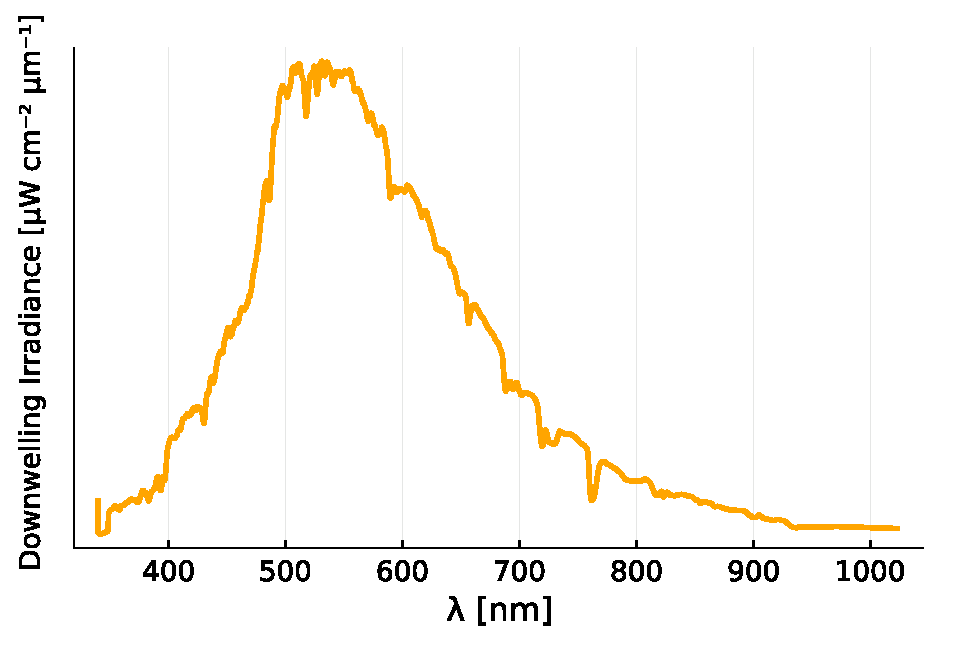
\includegraphics[width=10.5 cm]{images/spectra/solar_irradiance.eps}
\caption{Downwelling Irradiance captured via an upward facing spectrometer.\label{irradiancePlot}}
\end{figure}   

\begin{figure}[H]
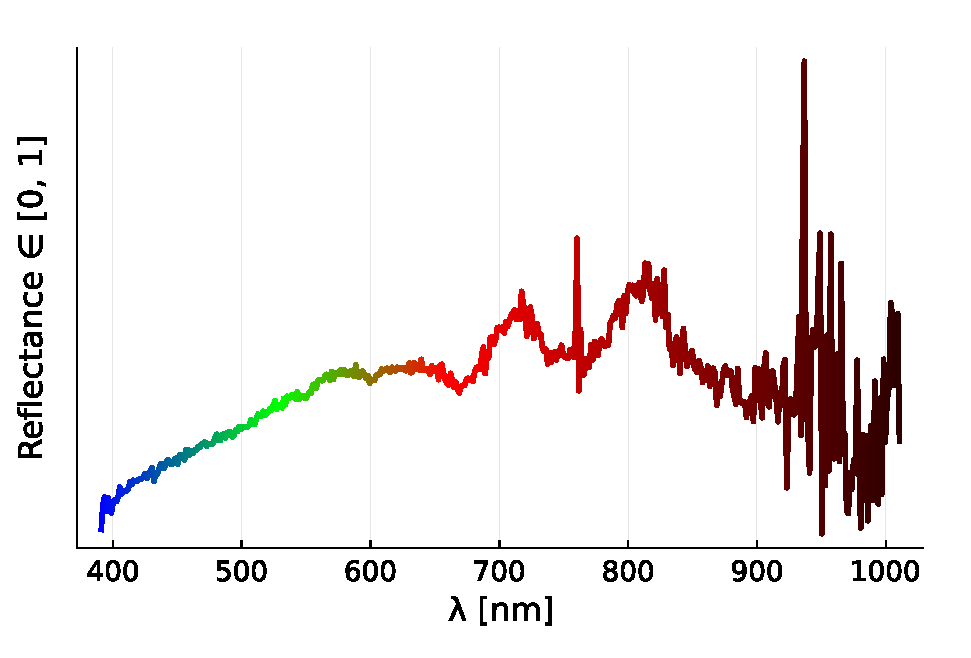
\includegraphics[width=10.5 cm]{images/spectra/reflectance_rainbow.eps}
\caption{Single pixel reflectance spectrum created by combining \ref{radiancePlot} with \ref{irradiancePlot}.\label{radiancePlot}}
\end{figure}   


\begin{equation}
    R = \pi \frac{L}{E}
\end{equation}


\subsection{Georectification}
paper by Muller \cite{GeorectificationMuller} \\ 
paper by Baumker \cite{GeorectificationBaumker} \\ 
paper by Mostafa \cite{GeorectificationMostafa} \\ 


NOTE: need to double check \cite{GeorectificationMuller} for convention used ($\Phi$ vs $\phi$) 

Heading correction due to longitude deviation in UTM system: 
\begin{equation}
    \kappa_{\text{geodetic}} = \kappa_{\text{geographic}}-\tan^{-1}\left( \sin\Phi \tan(\lambda-\lambda_{cm}) \right)
\end{equation}

scale factor: 
\begin{equation}
    s = \frac{z_{\text{sensor}}-z_{\text{ground}}}{f}
\end{equation}

\begin{equation}
    \begin{pmatrix}
    x \\ y \\ z
    \end{pmatrix}_{\text{Object}}^{\text{UTM}} = 
    f_{\text{geo}}^{\text{UTM}}\begin{pmatrix}
    \lambda \\ 
    \Phi \\ 
    z
    \end{pmatrix}_{\text{GPS}}^{\text{geo}} + sT_{\text{IMU}}^{\text{UTM}}R_{\text{sensor}}^{\text{IMU}}(\kappa, \phi, \omega)\begin{pmatrix}
    0 \\ 
    y_i \\ 
    f
    \end{pmatrix}_{\text{object}}^{\text{sensor}}
\end{equation}


\begin{figure}[H]
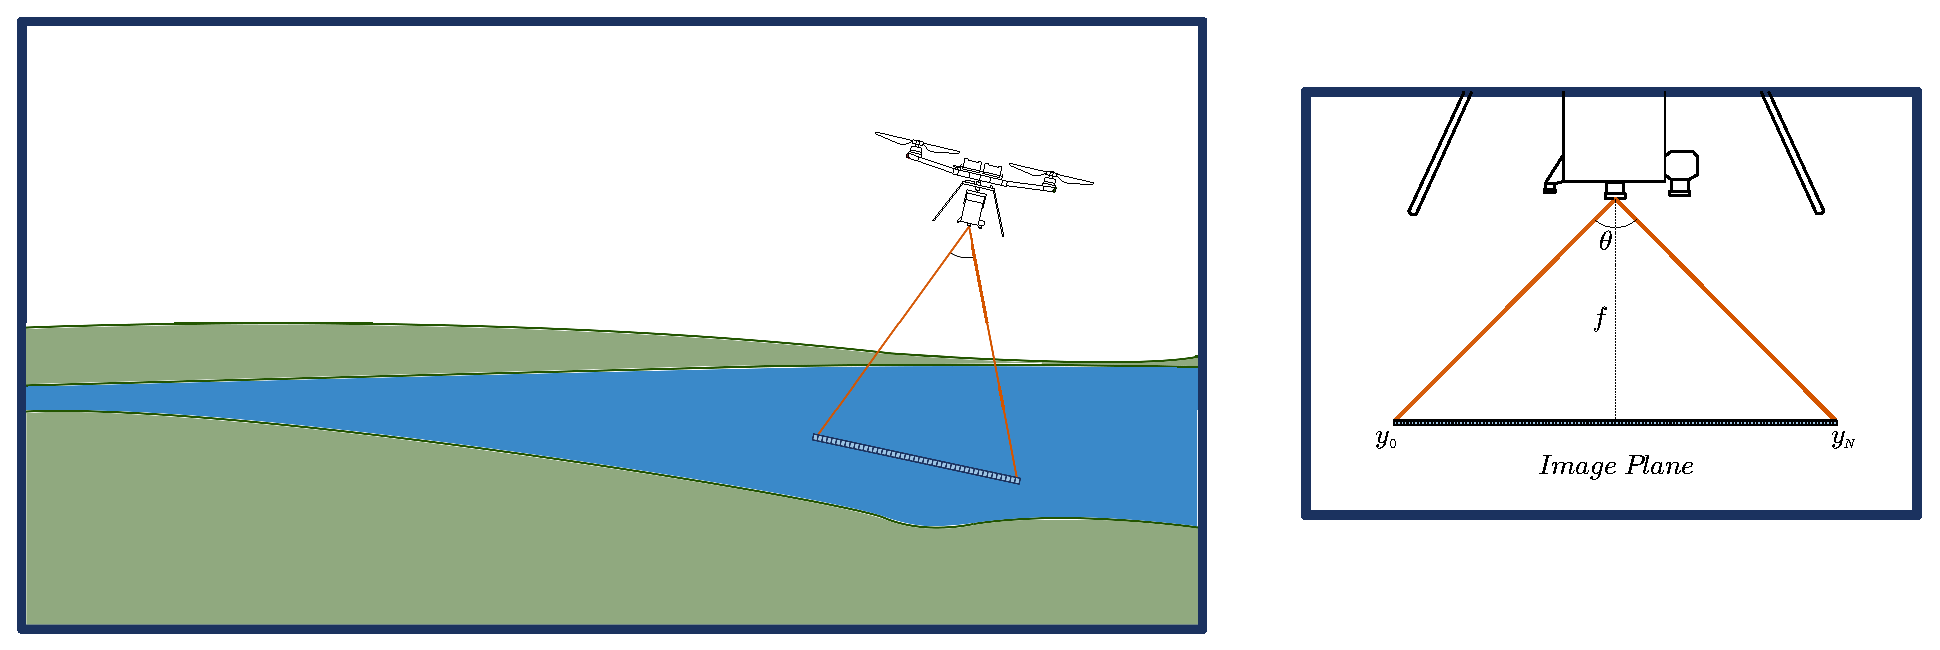
\includegraphics[width=10.5 cm]{images/georectification/georectification.eps}
\caption{Diagram of .\label{georectification1}}
\end{figure}   



\subsection{In-situ Data Collection via Robotic Sentinels}

autonomous boat website \cite{Otter}


\subsubsection{data collection process}
\subsubsection{Data Collocation}

\subsubsection{CO}
\subsubsection{CDOM}
\subsubsection{HDO}
\subsubsection{$Na^{+}$}
\subsubsection{$Ca^{2+}$}
\subsubsection{Other Targets}

\subsubsection{Feature Engineering with Remote Sensing Indices}
include discussion of PCA as well as Standardization


\subsection{Exploratory Data Analysis}
\subsubsection{Variable Correlations}

\begin{figure}[H]
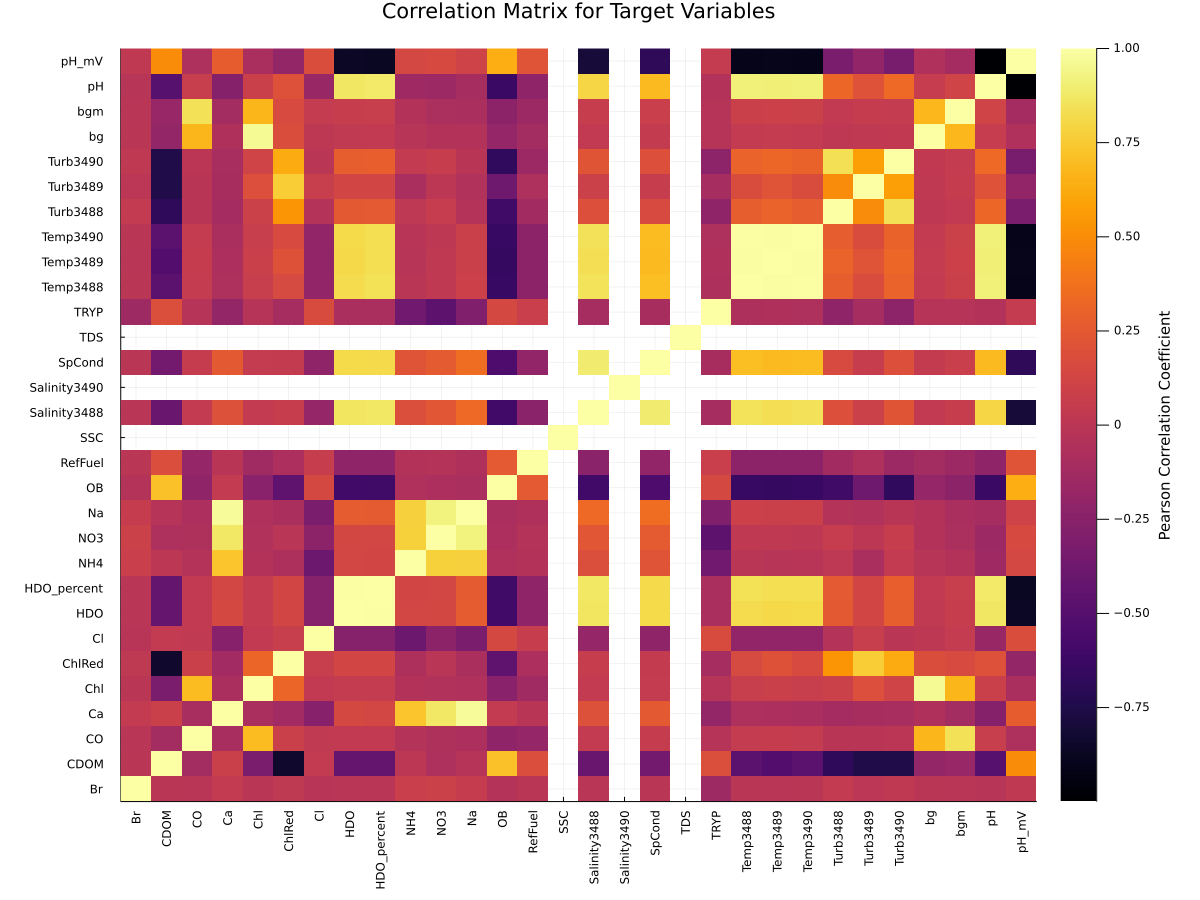
\includegraphics[width=10.5 cm]{images/correlation/target_cor.png}
\caption{Correlation Matrix for Target variables measured by the boat.\label{target_cor}}
\end{figure}   

\begin{figure}[H]
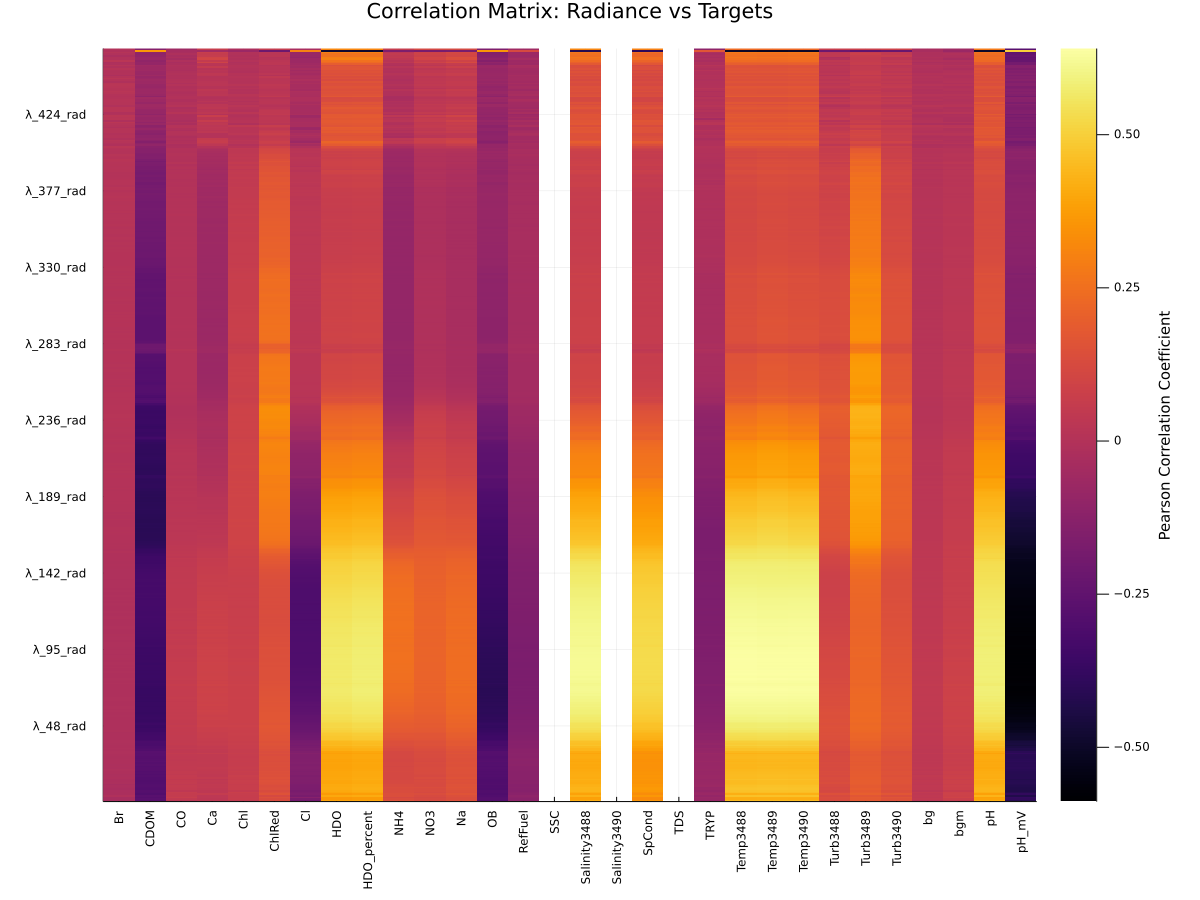
\includegraphics[width=10.5 cm]{images/correlation/radiance_cor.png}
\caption{Correlation Matrix for Radiance measurements versus Target Variables.\label{rad_cor}}
\end{figure}   

\begin{figure}[H]
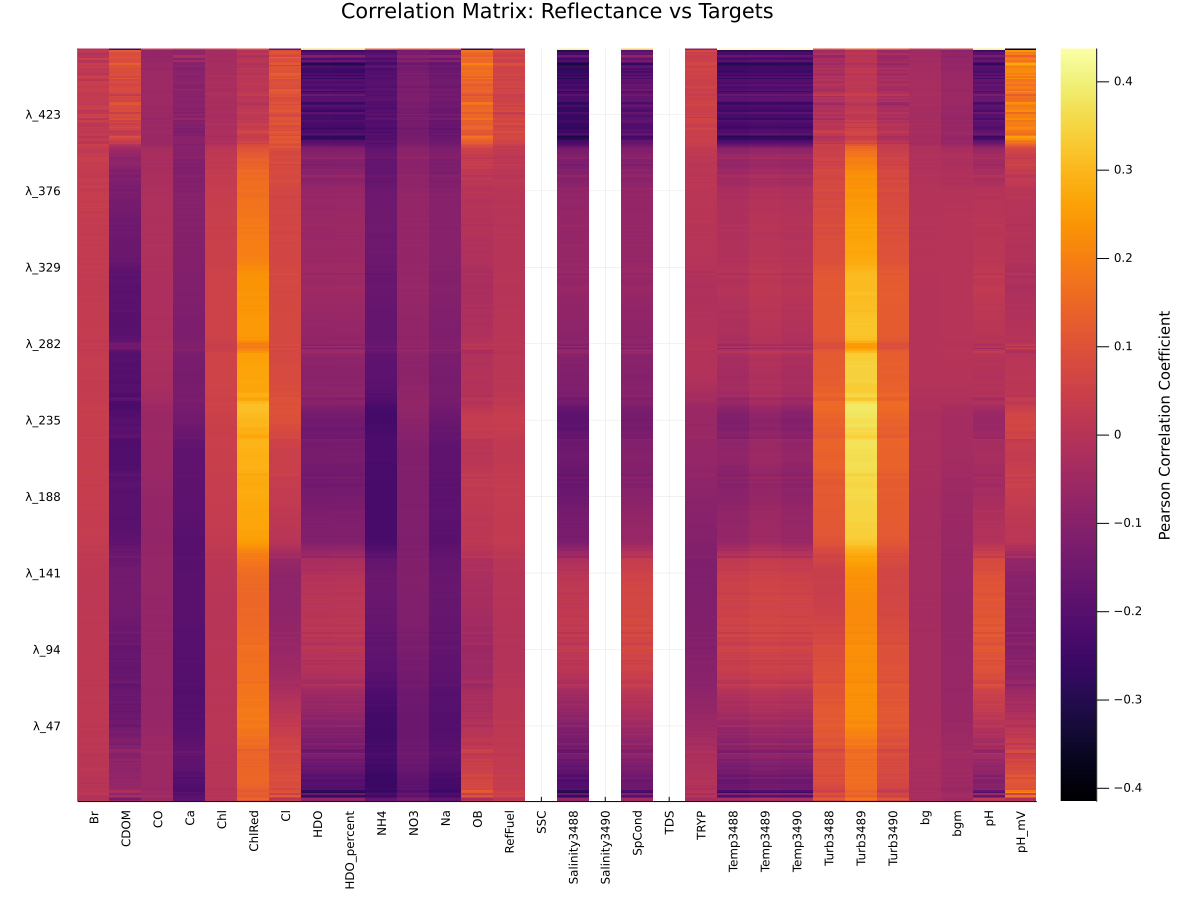
\includegraphics[width=10.5 cm]{images/correlation/reflectance_cor.png}
\caption{Correlation Matrix for Reflectance measurements versus Target Variables.\label{ref_cor}}
\end{figure}   

\begin{figure}[H]
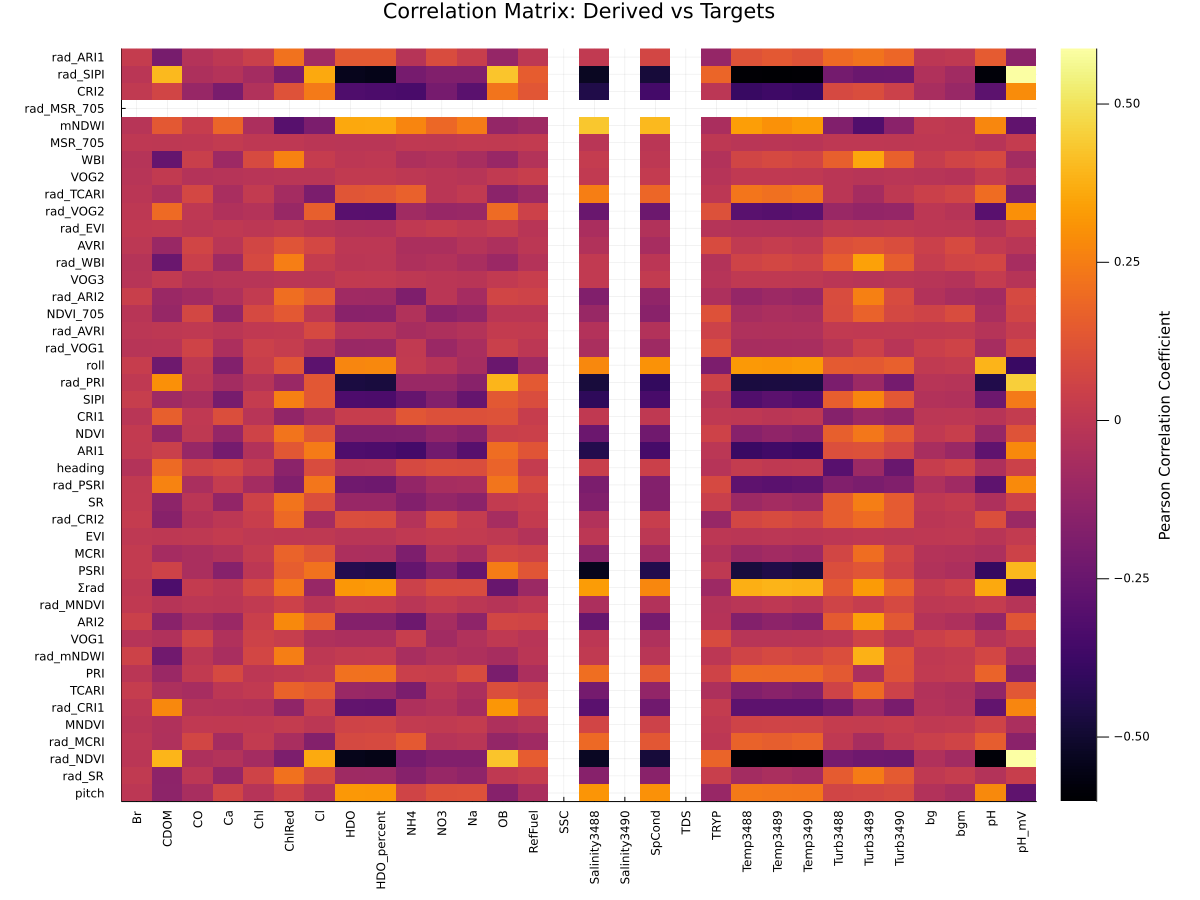
\includegraphics[width=10.5 cm]{images/correlation/derived_cor.png}
\caption{Correlation Matrix for derived measurements versus Target Variables.\label{derived_cor}}
\end{figure}   


\subsubsection{Unsupervised Classification}
\begin{figure}[H]
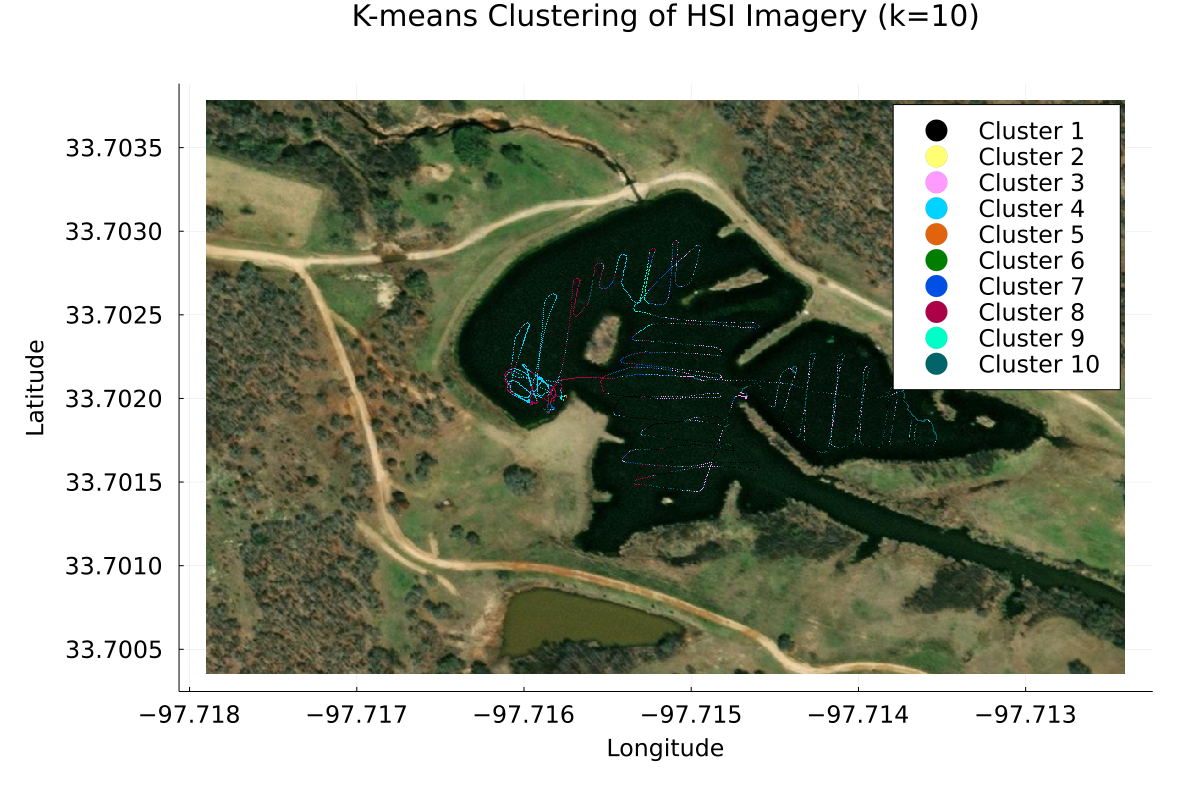
\includegraphics[width=11 cm]{images/unsupervised/clustering.png}
\caption{Unsupervised clustering of hyper-spectral image data using the K-means algorithm.\label{clustering}}
\end{figure}   


\subsection{Machine Learning}



\subsubsection{Machine Learning Models}
include Linear Models, Neural Networks, Decision Trees, Bagging, Boosting, and Stacking\\

The field of Machine Learning has seen the invention of a plethora of models able to perform inference for regression tasks. Naturally, this leads to the challenge of evaluating which model is best for a given problem. In 1992 David Wolpert developed the notion of Stacked Generalization to divorce arbitrary human choice from the model selection process. [1] The key idea is as follows: fit an instance of each model compatible with your dataset. Each model learns different features of the data so that an adjudicating model (called the super-learner) can then be trained to map the predictions from each individual learner to a final output prediction. This is incredibly easy to accomplish in the Julia programming language via the MLJ machine learning framework [2]. We train a variety of learners including artificial neural networks, bagged decision trees, boosted decision trees, polynomial regressors, quantile regressors, LASSO regressors, and K-nearest-neighbors regressors. To ensure proper data hygiene, individual learners are first trained on separate cross validation folds so as not to bias the super-learner. After training the super-learner, each individual model is then trained on the full dataset to produce the best possible model.


paper on stacking \cite{ModelStacking}

\subsection{Model Analysis}
aleatoric and epistemic uncertainty

The black-box nature most machine learning methods makes it difficult to consider how errors propagate through a trained model during the inference process. For many problems such as image classification this is not an issue, however, in physical sensing error considerations are vital to establish detection limits and prediction confidence. Typically, there are three considerations we must make: measurement uncertainty– how much we can trust our model’s inputs, measurement representativeness– how well each data point represents data within a local neighborhood, and model error– how far the prediction is from the true value. Machine learning models are typically trained to minimize the model error. The Julia programming language makes it possible to handle all three. 


To address measurement uncertainty, we take advantage of Julia’s advanced automatic differentiation capabilities to enable differentiable programming (∂P). This means that we can take derivatives of our trained ML model with respect to each input feature to perform a sensitivity analysis. The final output uncertainty is then given via linear error propagation theory. [5]

Measurement representativeness can be trickier to handle. For example, in fluids it is common for two species to form a mixing layer that presents as a sharp discontinuity in measurement values. To quantify the degree to which neighboring points diverge we compute the average deviation across input measurements in a neighborhood around each data sample. This information can then be presented with model outputs to identify the regions where our model is valid. Similarly for ensemble ML models we compute the prediction deviation across all base learners to identify the representativeness of a data sample. Inputs that cause a large spread in base learner predictions indicate low representativeness in the training set. This analysis can then be used to plan further data collection missions that minimize time spent collecting data we have already present in our models. 

\subsubsection{Uncertainty Propagation via ($\partial P$)}

\subsubsection{Feature Ranking via SHAP values}

shape value paper used in ShapML.jl \cite{SHAPvalues1}

\subsubsection{Data Representativeness}
i.e. the average deviation across pixels used average during collocation process.
Also, we can look at relative disagreement between model predictions in bagged ensemble. 

\section{Results}
\subsection{CO}

\begin{figure}[H]
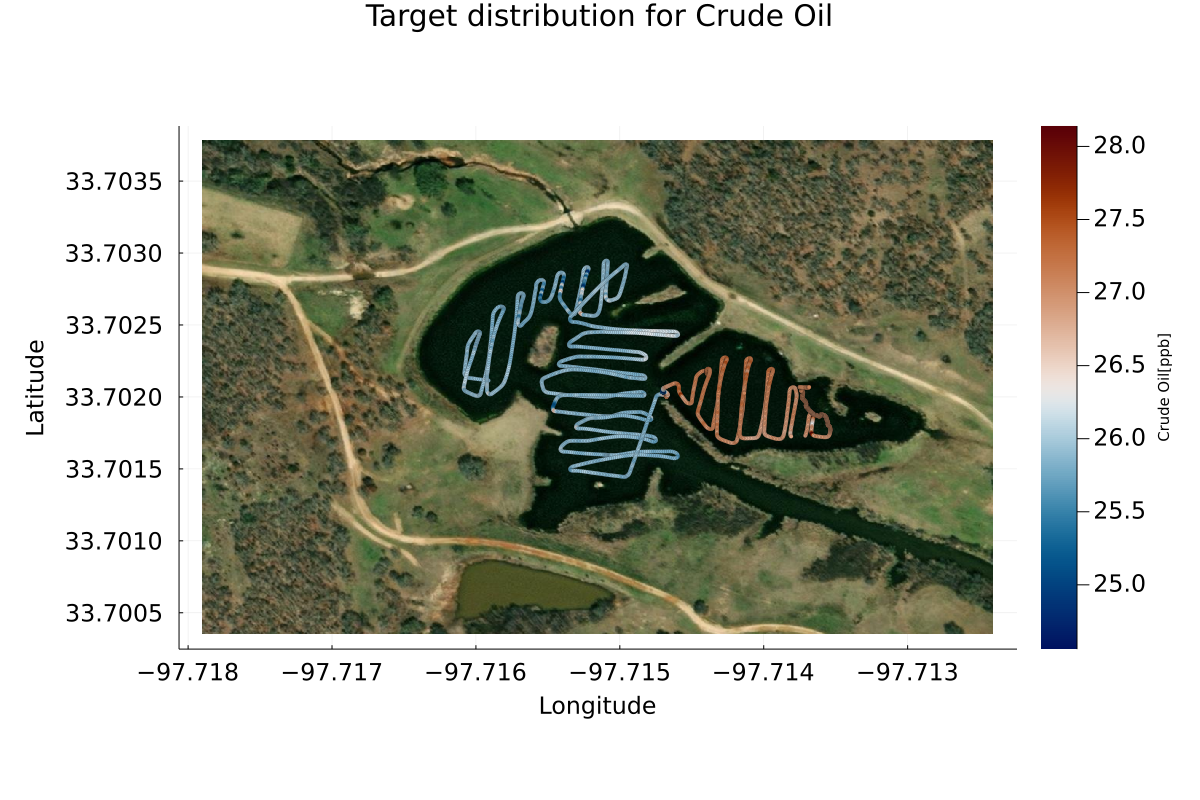
\includegraphics[width=10.5 cm]{images/CO/CO_dataMap.png}
\caption{Target distribution of CO at Scotty's Ranch.\label{CO_targetMap}}
\end{figure} 

\begin{figure}[H]
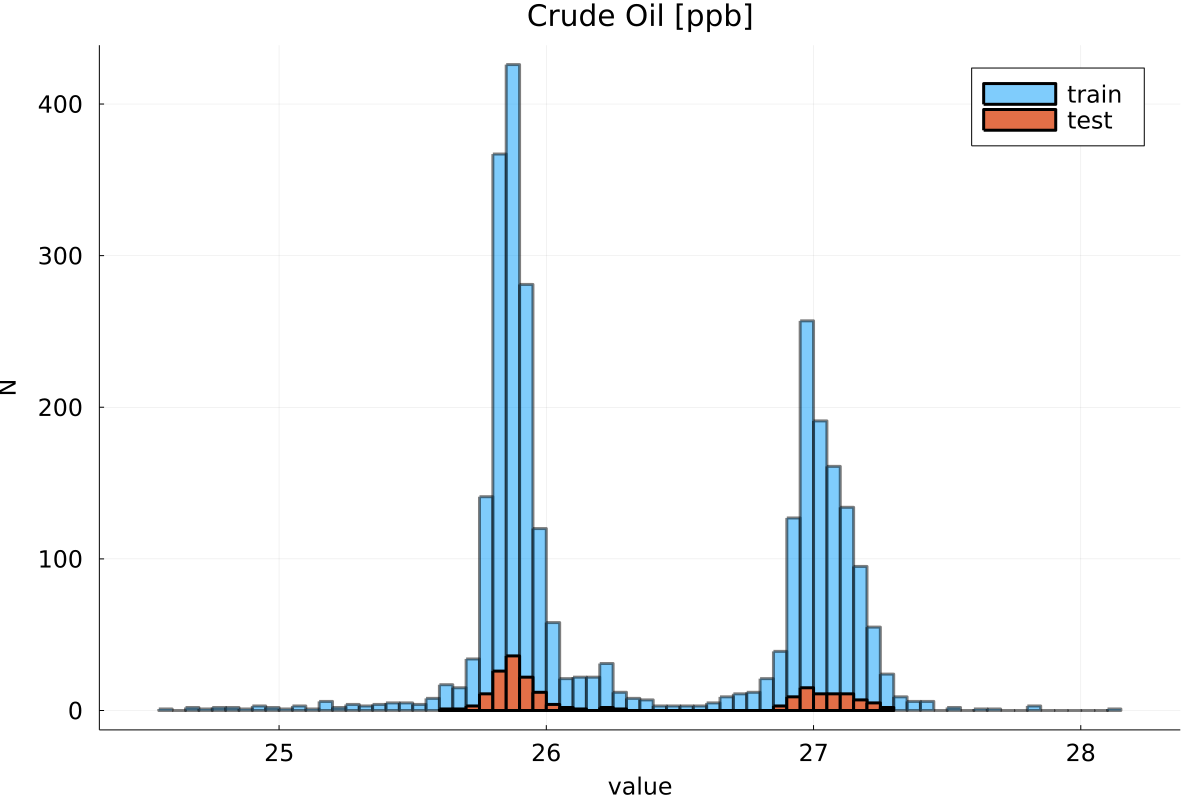
\includegraphics[width=10.5 cm]{images/CO/CO_train-test_hist.png}
\caption{Stratified train-test split for CO.\label{CO_trainTestHist}}
\end{figure}

\begin{figure}[H]
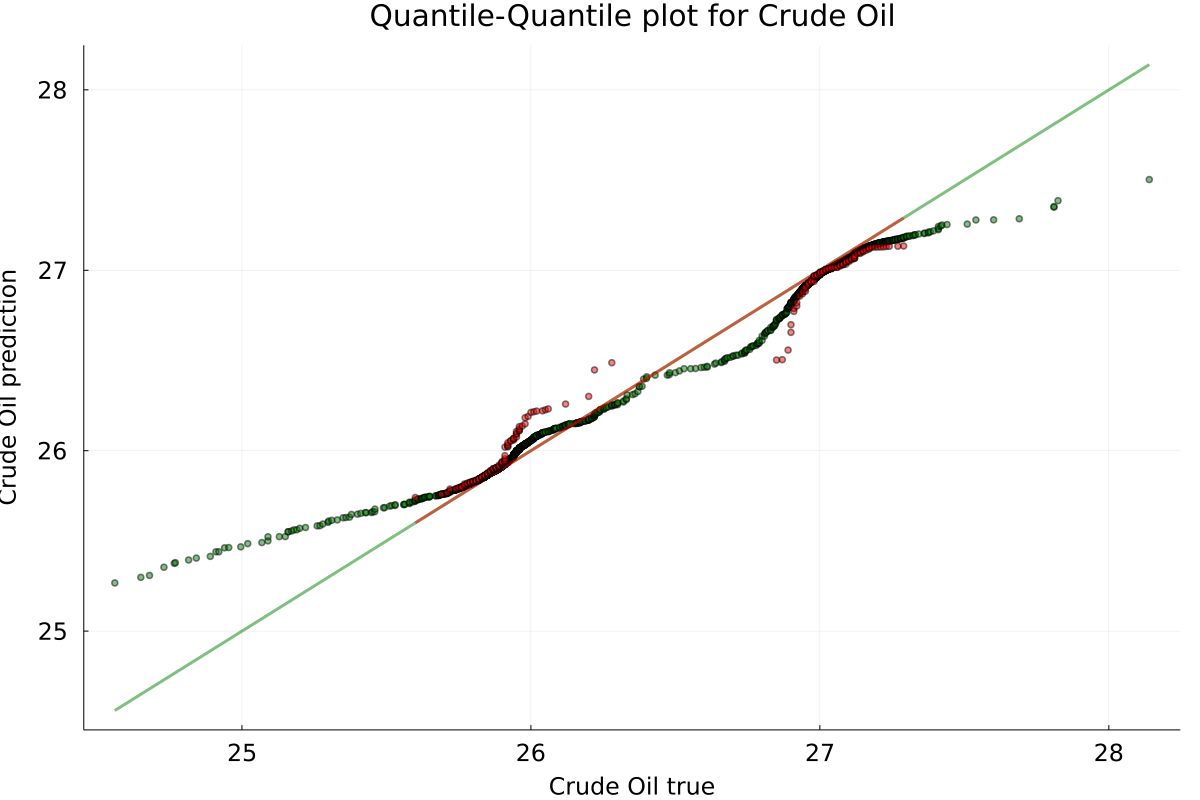
\includegraphics[width=10.5 cm]{images/CO/rfr_CO_qq.png}
\caption{Quantile-Quantile plot for CO random forest fit. \label{CO_trainTestHist}}
\end{figure}

\begin{figure}[H]
    \begin{adjustwidth}{-\extralength}{0cm}
    \centering
    \subfigure{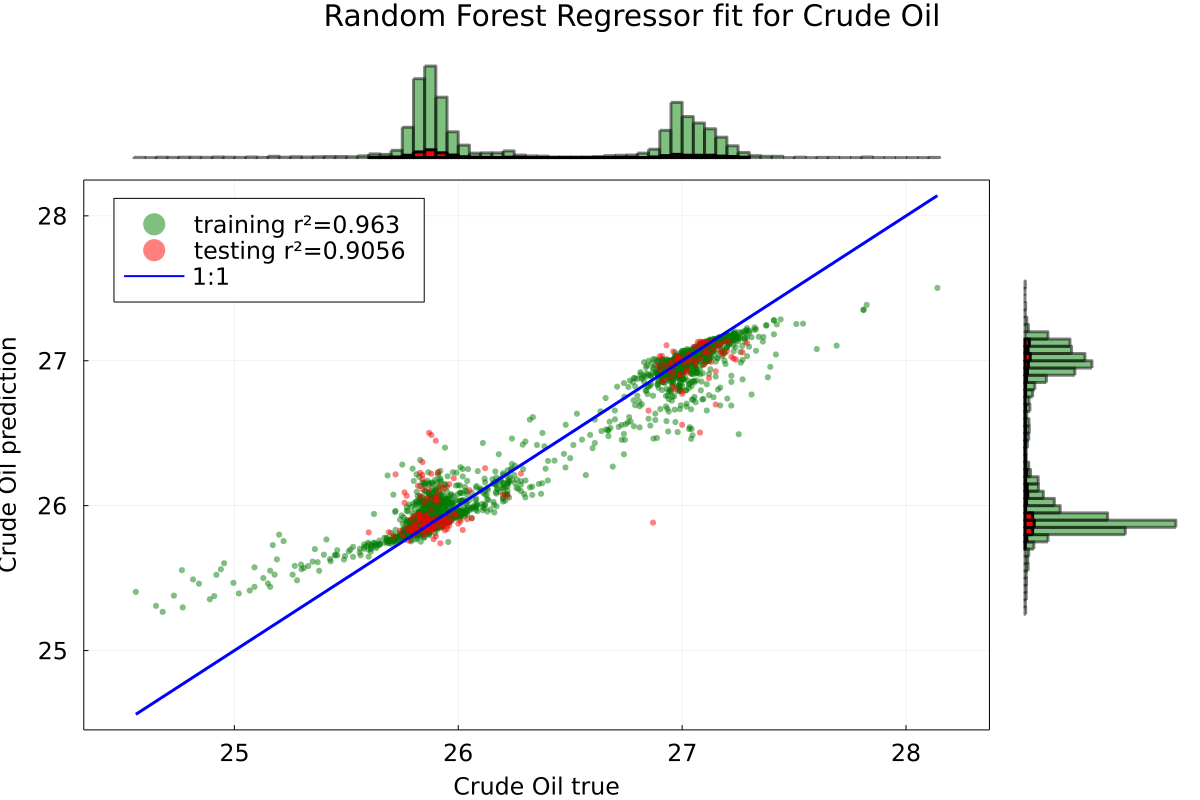
\includegraphics[width=0.5\textwidth]{images/CO/rfr_CO_scatter.png}}\qquad
    \subfigure{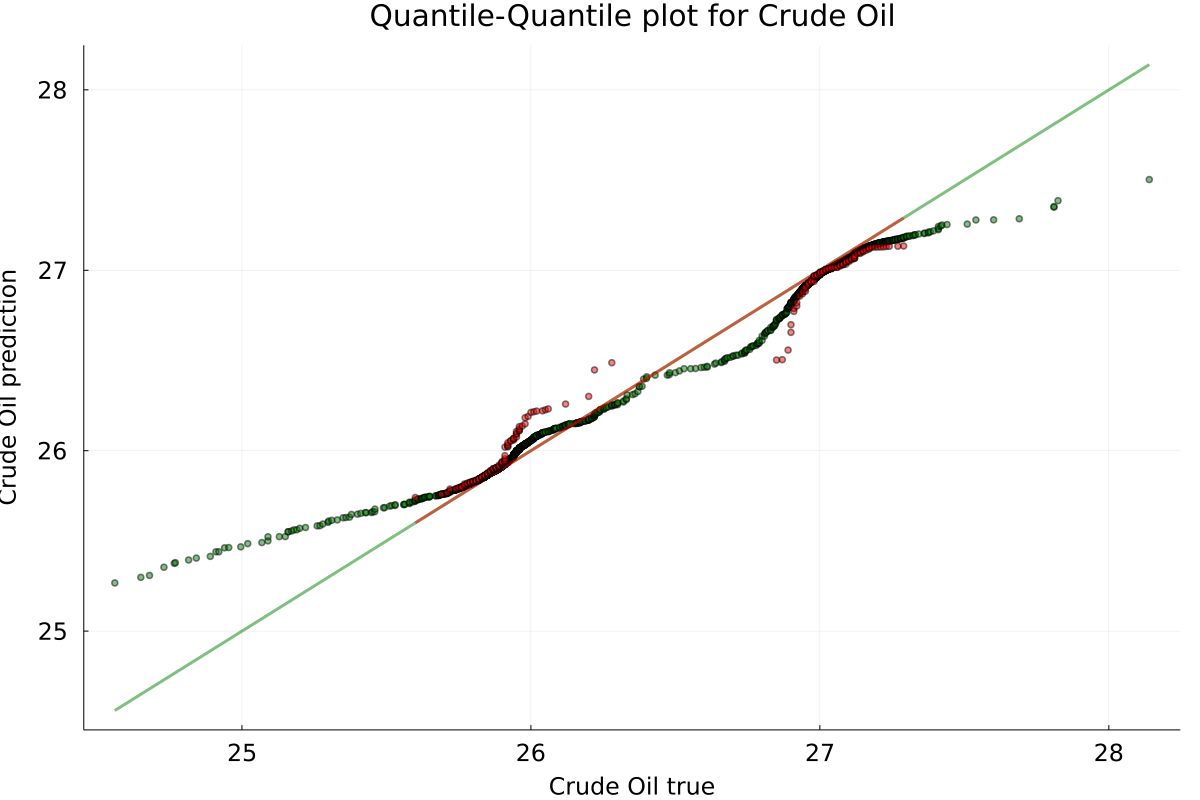
\includegraphics[width=0.5\textwidth]{images/CO/rfr_CO_qq.png}}
    \end{adjustwidth}
    \caption{(\textbf{a}) Scatterplot for the trained random forest Crudo Oil model. (\textbf{b}) Quantile-Quantile plot for the same fit.}
    \label{CO_fitresult}
\end{figure}

\begin{figure}[H]
    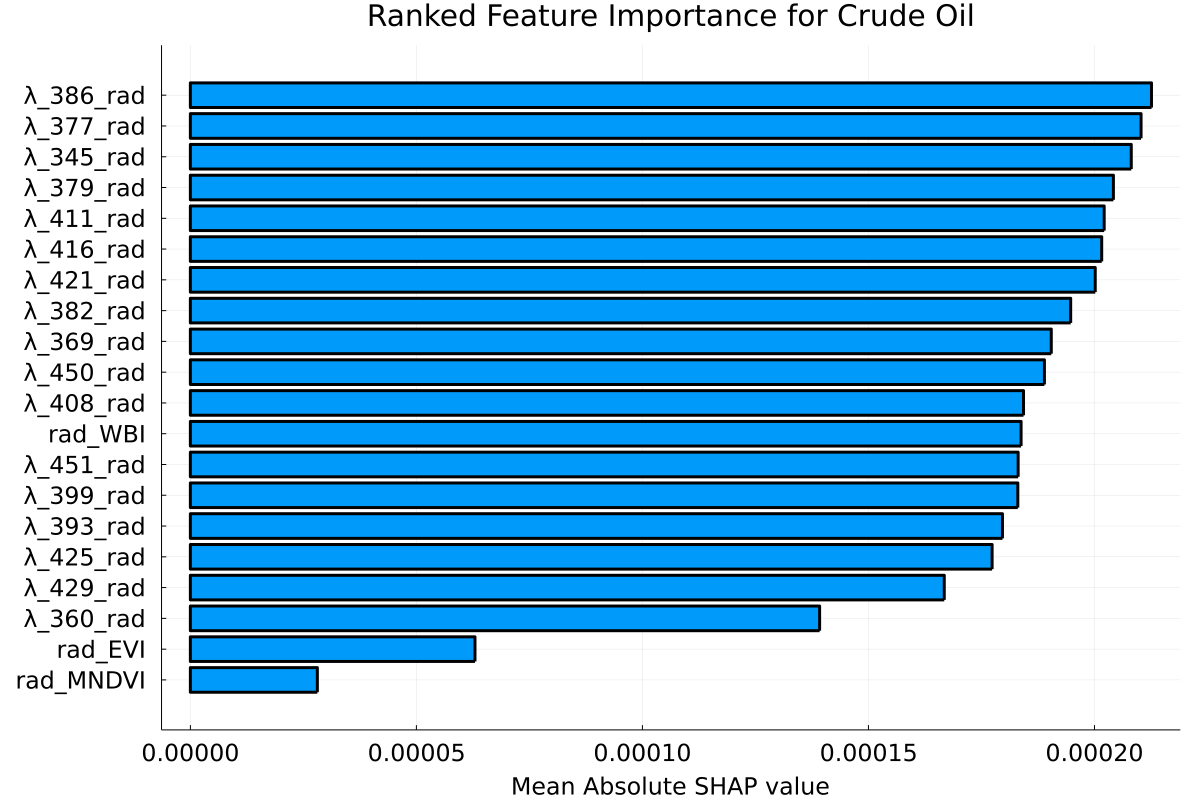
\includegraphics[width=10.5 cm]{images/CO/rfr_CO_featureImportance.png}
    \caption{Ranked feature importance for Crude Oil. Importance is determined via mean absolute SHAP value. \label{CO_shapely}}
\end{figure}



\section{Discussion}
\subsection{For-deployment Models}
\subsubsection{Random Forests}


\subsection{Limitations}
discuss viewing geometry and time of day

\subsection{Extensions and Future Work}
\subsubsection{Physics-informed machine learning}
\subsubsection{Data Augmentation}

\section{Conclusions}


%%%%%%%%%%%%%%%%%%%%%%%%%%%%%%%%%%%%%%%%%% 
\vspace{6pt} 

%%%%%%%%%%%%%%%%%%%%%%%%%%%%%%%%%%%%%%%%%%
%% optional
%\supplementary{The following are available online at \linksupplementary{s1}, Figure S1: title, Table S1: title, Video S1: title.}

% Only for the journal Methods and Protocols:
% If you wish to submit a video article, please do so with any other supplementary material.
% \supplementary{The following are available at \linksupplementary{s1}, Figure S1: title, Table S1: title, Video S1: title. A supporting video article is available at doi: link.} 

%%%%%%%%%%%%%%%%%%%%%%%%%%%%%%%%%%%%%%%%%%
\authorcontributions{For research articles with several authors, a short paragraph specifying their individual contributions must be provided. The following statements should be used ``Conceptualization, X.X. and Y.Y.; methodology, X.X.; software, X.X.; validation, X.X., Y.Y. and Z.Z.; formal analysis, X.X.; investigation, X.X.; resources, X.X.; data curation, X.X.; writing---original draft preparation, X.X.; writing---review and editing, X.X.; visualization, X.X.; supervision, X.X.; project administration, X.X.; funding acquisition, Y.Y. All authors have read and agreed to the published version of the manuscript.'', please turn to the  \href{http://img.mdpi.org/data/contributor-role-instruction.pdf}{CRediT taxonomy} for the term explanation. Authorship must be limited to those who have contributed substantially to the work~reported.}

\funding{Please add: ``This research received no external funding'' or ``This research was funded by NAME OF FUNDER grant number XXX.'' and  and ``The APC was funded by XXX''. Check carefully that the details given are accurate and use the standard spelling of funding agency names at \url{https://search.crossref.org/funding}, any errors may affect your future funding.}

\institutionalreview{In this section, please add the Institutional Review Board Statement and approval number for studies involving humans or animals. Please note that the Editorial Office might ask you for further information. Please add ``The study was conducted according to the guidelines of the Declaration of Helsinki, and approved by the Institutional Review Board (or Ethics Committee) of NAME OF INSTITUTE (protocol code XXX and date of approval).'' OR ``Ethical review and approval were waived for this study, due to REASON (please provide a detailed justification).'' OR ``Not applicable'' for studies not involving humans or animals. You might also choose to exclude this statement if the study did not involve humans or animals.}

\informedconsent{Any research article describing a study involving humans should contain this statement. Please add ``Informed consent was obtained from all subjects involved in the study.'' OR ``Patient consent was waived due to REASON (please provide a detailed justification).'' OR ``Not applicable'' for studies not involving humans. You might also choose to exclude this statement if the study did not involve humans.

Written informed consent for publication must be obtained from participating patients who can be identified (including by the patients themselves). Please state ``Written informed consent has been obtained from the patient(s) to publish this paper'' if applicable.}

\dataavailability{In this section, please provide details regarding where data supporting reported results can be found, including links to publicly archived datasets analyzed or generated during the study. Please refer to suggested Data Availability Statements in section ``MDPI Research Data Policies'' at \url{https://www.mdpi.com/ethics}. You might choose to exclude this statement if the study did not report any data.} 

\acknowledgments{In this section you can acknowledge any support given which is not covered by the author contribution or funding sections. This may include administrative and technical support, or donations in kind (e.g., materials used for experiments).}

\conflictsofinterest{Declare conflicts of interest or state ``The authors declare no conflict of interest.'' Authors must identify and declare any personal circumstances or interest that may be perceived as inappropriately influencing the representation or interpretation of reported research results. Any role of the funders in the design of the study; in the collection, analyses or interpretation of data; in the writing of the manuscript, or in the decision to publish the results must be declared in this section. If there is no role, please state ``The funders had no role in the design of the study; in the collection, analyses, or interpretation of data; in the writing of the manuscript, or in the decision to publish the~results''.} 

%% Optional
\sampleavailability{Samples of the compounds ... are available from the authors.}

%%%%%%%%%%%%%%%%%%%%%%%%%%%%%%%%%%%%%%%%%%
%% Only for journal Encyclopedia
%\entrylink{The Link to this entry published on the encyclopedia platform.}

%%%%%%%%%%%%%%%%%%%%%%%%%%%%%%%%%%%%%%%%%%
%% Optional
\abbreviations{Abbreviations}{
The following abbreviations are used in this manuscript:\\

\noindent 
\begin{tabular}{@{}ll}
MDPI & Multidisciplinary Digital Publishing Institute\\
DOAJ & Directory of open access journals\\
TLA & Three letter acronym\\
LD & Linear dichroism
\end{tabular}}

%%%%%%%%%%%%%%%%%%%%%%%%%%%%%%%%%%%%%%%%%%
%% Optional
\appendixtitles{no} % Leave argument "no" if all appendix headings stay EMPTY (then no dot is printed after "Appendix A"). If the appendix sections contain a heading then change the argument to "yes".
\appendixstart
\appendix
\section[\appendixname~\thesection]{}
\subsection[\appendixname~\thesubsection]{}
The appendix is an optional section that can contain details and data supplemental to the main text---for example, explanations of experimental details that would disrupt the flow of the main text but nonetheless remain crucial to understanding and reproducing the research shown; figures of replicates for experiments of which representative data are shown in the main text can be added here if brief, or as Supplementary Data. Mathematical proofs of results not central to the paper can be added as an appendix.

\begin{table}[H] 
\caption{This is a table caption.\label{tab5}}
\newcolumntype{C}{>{\centering\arraybackslash}X}
\begin{tabularx}{\textwidth}{CCC}
\toprule
\textbf{Title 1}	& \textbf{Title 2}	& \textbf{Title 3}\\
\midrule
Entry 1		& Data			& Data\\
Entry 2		& Data			& Data\\
\bottomrule
\end{tabularx}
\end{table}

\section[\appendixname~\thesection]{}
All appendix sections must be cited in the main text. In the appendices, Figures, Tables, etc. should be labeled, starting with ``A''---e.g., Figure A1, Figure A2, etc.

%%%%%%%%%%%%%%%%%%%%%%%%%%%%%%%%%%%%%%%%%%
%\printendnotes[custom] % Un-comment to print a list of endnotes
\begin{adjustwidth}{-\extralength}{0cm}
\reftitle{References}

% Please provide either the correct journal abbreviation (e.g. according to the “List of Title Word Abbreviations” http://www.issn.org/services/online-services/access-to-the-ltwa/) or the full name of the journal.
% Citations and References in Supplementary files are permitted provided that they also appear in the reference list here. 

%=====================================
% References, variant A: external bibliography
% =====================================
\bibliography{references}

% If authors have biography, please use the format below
%\section*{Short Biography of Authors}
%\bio
%{\raisebox{-0.35cm}{\includegraphics[width=3.5cm,height=5.3cm,clip,keepaspectratio]{Definitions/author1.pdf}}}
%{\textbf{Firstname Lastname} Biography of first author}
%
%\bio
%{\raisebox{-0.35cm}{\includegraphics[width=3.5cm,height=5.3cm,clip,keepaspectratio]{Definitions/author2.jpg}}}
%{\textbf{Firstname Lastname} Biography of second author}

% For the MDPI journals use author-date citation, please follow the formatting guidelines on http://www.mdpi.com/authors/references
% To cite two works by the same author: \citeauthor{ref-journal-1a} (\citeyear{ref-journal-1a}, \citeyear{ref-journal-1b}). This produces: Whittaker (1967, 1975)
% To cite two works by the same author with specific pages: \citeauthor{ref-journal-3a} (\citeyear{ref-journal-3a}, p. 328; \citeyear{ref-journal-3b}, p.475). This produces: Wong (1999, p. 328; 2000, p. 475)

%%%%%%%%%%%%%%%%%%%%%%%%%%%%%%%%%%%%%%%%%%
%% for journal Sci
%\reviewreports{\\
%Reviewer 1 comments and authors’ response\\
%Reviewer 2 comments and authors’ response\\
%Reviewer 3 comments and authors’ response
%}
%%%%%%%%%%%%%%%%%%%%%%%%%%%%%%%%%%%%%%%%%%
\end{adjustwidth}
\end{document}

